%% LyX 2.2.2 created this file.  For more info, see http://www.lyx.org/.
%% Do not edit unless you really know what you are doing.
\documentclass[11pt,british]{scrartcl}
\usepackage{lmodern}
\renewcommand{\sfdefault}{lmss}
\renewcommand{\ttdefault}{lmtt}
\usepackage[T1]{fontenc}
\usepackage[latin9]{inputenc}
\usepackage[a4paper]{geometry}
\geometry{verbose,bmargin=2.5cm}
\setcounter{secnumdepth}{4}
\setcounter{tocdepth}{4}
\setlength{\parindent}{0bp}
\usepackage{babel}
\usepackage{array}
\usepackage{longtable}
\usepackage{float}
\usepackage{textcomp}
\usepackage{enumitem}
\usepackage{amssymb}
\usepackage{graphicx}
\usepackage[unicode=true,pdfusetitle,
 bookmarks=true,bookmarksnumbered=false,bookmarksopen=false,
 breaklinks=true,pdfborder={0 0 0},pdfborderstyle={},backref=false,colorlinks=false]
 {hyperref}

\makeatletter

%%%%%%%%%%%%%%%%%%%%%%%%%%%%%% LyX specific LaTeX commands.
%% Because html converters don't know tabularnewline
\providecommand{\tabularnewline}{\\}

%%%%%%%%%%%%%%%%%%%%%%%%%%%%%% Textclass specific LaTeX commands.
\newlength{\lyxlabelwidth}      % auxiliary length 

%%%%%%%%%%%%%%%%%%%%%%%%%%%%%% User specified LaTeX commands.
\usepackage{microtype}
\usepackage{eurosym}
\addtokomafont{disposition}{\rmfamily}
\usepackage[headsepline]{scrlayer-scrpage}
\clearpairofpagestyles
\ohead{DD}
\chead{\pagemark}
\ihead{\headmark}
\automark[]{section}
\renewcommand*\pagemark{{\usekomafont{pagenumber}Page\nobreakspace\thepage}}
\addtokomafont{pageheadfoot}{\upshape}

\makeatother

\usepackage{listings}
\lstset{basicstyle={\ttfamily},
columns=fullflexible}
\begin{document}

\title{Design Document}

\author{Philippe Scorsolini,\\
Lorenzo Semeria,\\
Gabriele Vanoni}

\subject{Politecnico di Milano, A.Y. 2016/2017\\
M.Sc. Degree Programme in Computer Science and Engineering\\
Software Engineering 2 Project}

\maketitle
\pagebreak{}

\tableofcontents{}

\pagebreak{}

\section{Introduction}

\subsection{Purpose}

The purpose of this document is to give the detailed structure of
PowerEnJoy software system.

So we try to give developers a clear representation of:
\begin{itemize}
\item The high level architecture of the system.
\item The design patterns applied in order to achieve our specific necessities.
\item The main components and the interfaces they provide.
\item The Runtime behaviour.
\end{itemize}

\subsection{Scope}

PowerEnJoy project aims to provide users and operators with means
to use the system services they need and they are supposed to have
access to. It also provides an API for external services to access
the system with ``operator'' rights, in order to allow call center
operators to interface with the system.

The system allows: 
\begin{itemize}
\item Users to manage their personal data through both a web and a mobile
app and Active Users to manage reservations.
\item Callcenter's operators to manage assistance tickets via the API. The
tickets will then be managed internally by PowerEnJoy.
\item PowerEnjoy's operators to manage the open assistance tickets, take
them in charge and update car's and user's data accordingly.
\end{itemize}
The system architecture shall guarantee future proof scalability and
allow subsequent improvements and general reliability.

\subsection{Abbreviations, Definitions and Acronyms}

\subsubsection{Abbreviations:}
\begin{itemize}
\item Gn: the n-th Goal
\item An: the n-th Assumption
\item Rn: the n-th Requirement
\end{itemize}

\subsubsection{Acronyms}
\begin{itemize}
\item CC: Credit Card
\item DL: Driving Licence
\item AU: Active User
\end{itemize}

\subsubsection{Definitions}
\begin{itemize}
\item Visitor: person that may not be registered to the system or not logged
in.
\item User: a registered and logged in Visitor, that may be still waiting
for his information to be verified.
\item Active User: a User whose data (CC, DL) have been verified. (Shares
all User's characteristics)
\item Safe Zone: predefined zones where parking is allowed, parking is forbidden
in any other zone.
\item Park: park the car in the safe zone and terminate the rental.
\end{itemize}
\pagebreak{}

\section{Architectural Design}

\subsection{Design Process}

In this subsection we'll try to give an overview of the process that
brought to the final design chosen for the system, underlining the
reasons that motivated our main choices in a mixed top-down/bottom-up
approach. The more detailed description of the system will be given
in the remainder of the document.

Initially, given the goals and the requirements we have depicted in
the RASD, we have decided to adopt a three tier client-server architecture
to be able to manage different clients and to decouple the three layers,
this choice was trivial given the nature and the needs of our system,
not so trivial was the choice of adopting a thin client in order to
not have any performance constraint on the client's hardware to maximize
the possibility of adoption by the user of our service. 

Then we have started aggregating the different requirements in much
granular components, trying to follow a single responsibility principle,
as can be seen in section 5. So we have depicted the following components
as part of the second tier on the server side of our system: 
\begin{itemize}
\item Client Handler: orchestrates the needed services for the clients,
translating client's requests to the server and returning the needed
data.
\item Authentication Manager: ensures that only authorised users are able
to perform ``restricted'' actions as well as checking login credentials.
\item Registration Manager: manages the registration of new users and the
update of registered users' data if needed.
\item Administration Module: grants PowerEnJoy's operators access to some
specific features needed to manage the assistance tickets they have
to take care of.
\item Model Manager: grants access to the data to the other components,
abstracting any kind of technology specific detail to the other services.
\item Car Manager: manages the physical cars providing other services with
the needed functionalities and informations.
\item Power Station Manager: manages the physical power stations' data and
functionalities.
\item Assistance Ticket Manager: grants the assistance callcenter, the operators
and the other services the APIs to manage the assistance tickets.
\item Reservation Manager: manages the whole reservation process for an
Active User from the reservation intention to the effective payment,
interacting with the external payment handler through his APIs.
\end{itemize}
\begin{figure}[H]
\hfill{}\includegraphics[width=0.5\linewidth]{\string"component lvl 2 - Page 1\string".pdf}\hfill{}

\caption{Component view derived from the Requirements analysis}
\end{figure}

Then we needed to find where our components could be deployed and
how we would have managed the communication between them, we could
have adopted a monolithic approach or take advantage of the well established
application server architecture, but that wouldn't have granted the
scalability and the independent deployment of the components we were
looking for, so we decided to go for a microservice oriented architecture.
This choice allowed us to take advantage of the growing number of
Platform-as-a-Service providers, so it seemed natural given the previous
choices to deploy our whole server side in the cloud, giving us the
ability to scale our application on need and abstracting us from any
hardware specific consideration in the future. 

To fully take advantage of this architectural style we have introduced
some components that will manage the life cycle of the deployed components:
\begin{itemize}
\item Discovery Service: gives to other services the references that allow
them to communicate with each other.
\item Binding Service: manages the queue binding for the services.i
\end{itemize}
\begin{figure}[H]
\hfill{}\includegraphics[width=0.5\linewidth]{\string"component lvl 2b\string".pdf}\hfill{}

\caption{Component view derived from the Requirements analysis and the decision
of microservice oriented architecture}
\end{figure}

Although we had decided to transform our three-tiered application
in a three-tiered cloud application, the problem of the communication
between our microservices still needed a solution, two options arose
as the most valuable of attention: a point-to-point communication
approach or a more centralized messaging/bus oriented one. These two
options where not linked to the choice of a cloud application, it
could have also be adopted in a server. The obvious advantages of
the first one with respect to the second where the absence of a clear
single point of failure and with that the absence of a possible bottleneck
in the central message bus, but the disadvantages such as the difficulty
of managing the whole system without a central coordinator and the
numerous APIs that such approach would have needed, but given the
previewed load of our system the advantage didn't seem really much
of an advantage and the disadvantage would have burdened the development
of the system. 

Checked some numbers of the actual load the of the third party message
broker could handle and the advantages of adopting one of them, we
have decided to adopt a centralized message broker that with a publish
subscribe pattern would manage the communication between the components
giving us as secondary effect the possibility to implement some advanced
load balancing techniques in the near future to better take advantage
of the pay-per-use approach the cloud provides.

\begin{figure}[H]
\hfill{}\includegraphics[width=0.5\linewidth]{\string"Component with message broker\string".pdf}\hfill{}

\caption{Component view derived from the message broker decision}
\end{figure}

After deciding the structure of the server side, we have focused on
the remainder part of the deployment diagram and depicted the counterpart
of the previous components outside the server, such as the software
that will be deployed inside the cars and the one for the powerstations
and the two clients' software accordingly to the RASD specifications.

Then we've tried to give a possible, but not mandatory, implementation
of the system, especially concerning the communication protocols that
could be used between the different parts of the system and the technologies
that could be used to implement them, in order to check the feasibility
of our choices. Java Enterprise Edition as implementation language
seemed the most adopted solution for this kind of systems and microservice-oriented
framework on top of JEE such as Spring Boot could ease the development
fitting most of our needs out of the box, even if our design choice
could give the development team of each service the freedom to choose
the most appropriate framework/language as long as the communication
protocol chosen is supported.

\subsection{Overview}

The system adopts a three tier architecture with a thin client represented
by web and mobile app, which allows users and operators to access
through a GUI the different functionalities of the system accordingly
to the type of client used. These clients are both managed by a specific
server-side ClientHandler offering the same interface to other server-side
services and handling appropriately the communication with the two
clients adopting in both cases an asynchronous implementation of the
RESTful APIs over HTTPS in JSON format in order to achieve complete
freedom of development-specific choices on both sides.

The second tier adopts a microservice oriented architecture with shared
database that, taking into account the unknown but supposedly not
massive load of the system in the near future, reduces the need of
synchronization between services. This allows to keep the structure
as simple as possible, allowing better performing solutions such as
``database per service'' or ``schema per service'' to be implemented
when needed. This tier will also manage the communication with the
cars and the power station around the city through OpenVPN and MQTT
protocols.

The third tier provides the previous one the necessary abstraction
on the storage technology chosen and will manage the concurrent access
to the database. In case a PaaS hosting service is chosen, this tier
will be managed by the provider.

The second and third tier are designed to be deployed on the cloud
in order to take advantage of the ``scale on need'' possibility
it gives. For this reason it has been designed as a micro service
architecture.

\begin{figure}[H]
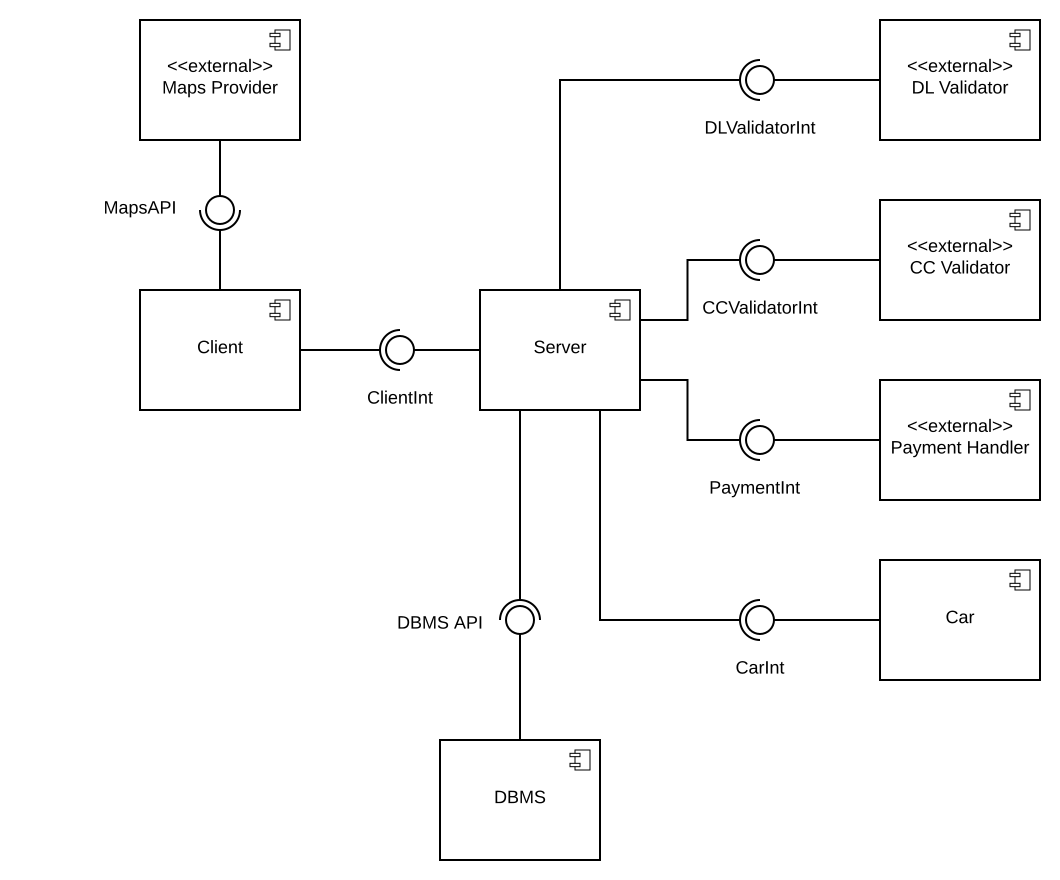
\includegraphics[width=1\textwidth]{OverView}

\caption{Component View overview}
\end{figure}


\subsection{Component View}

\begin{figure}[H]
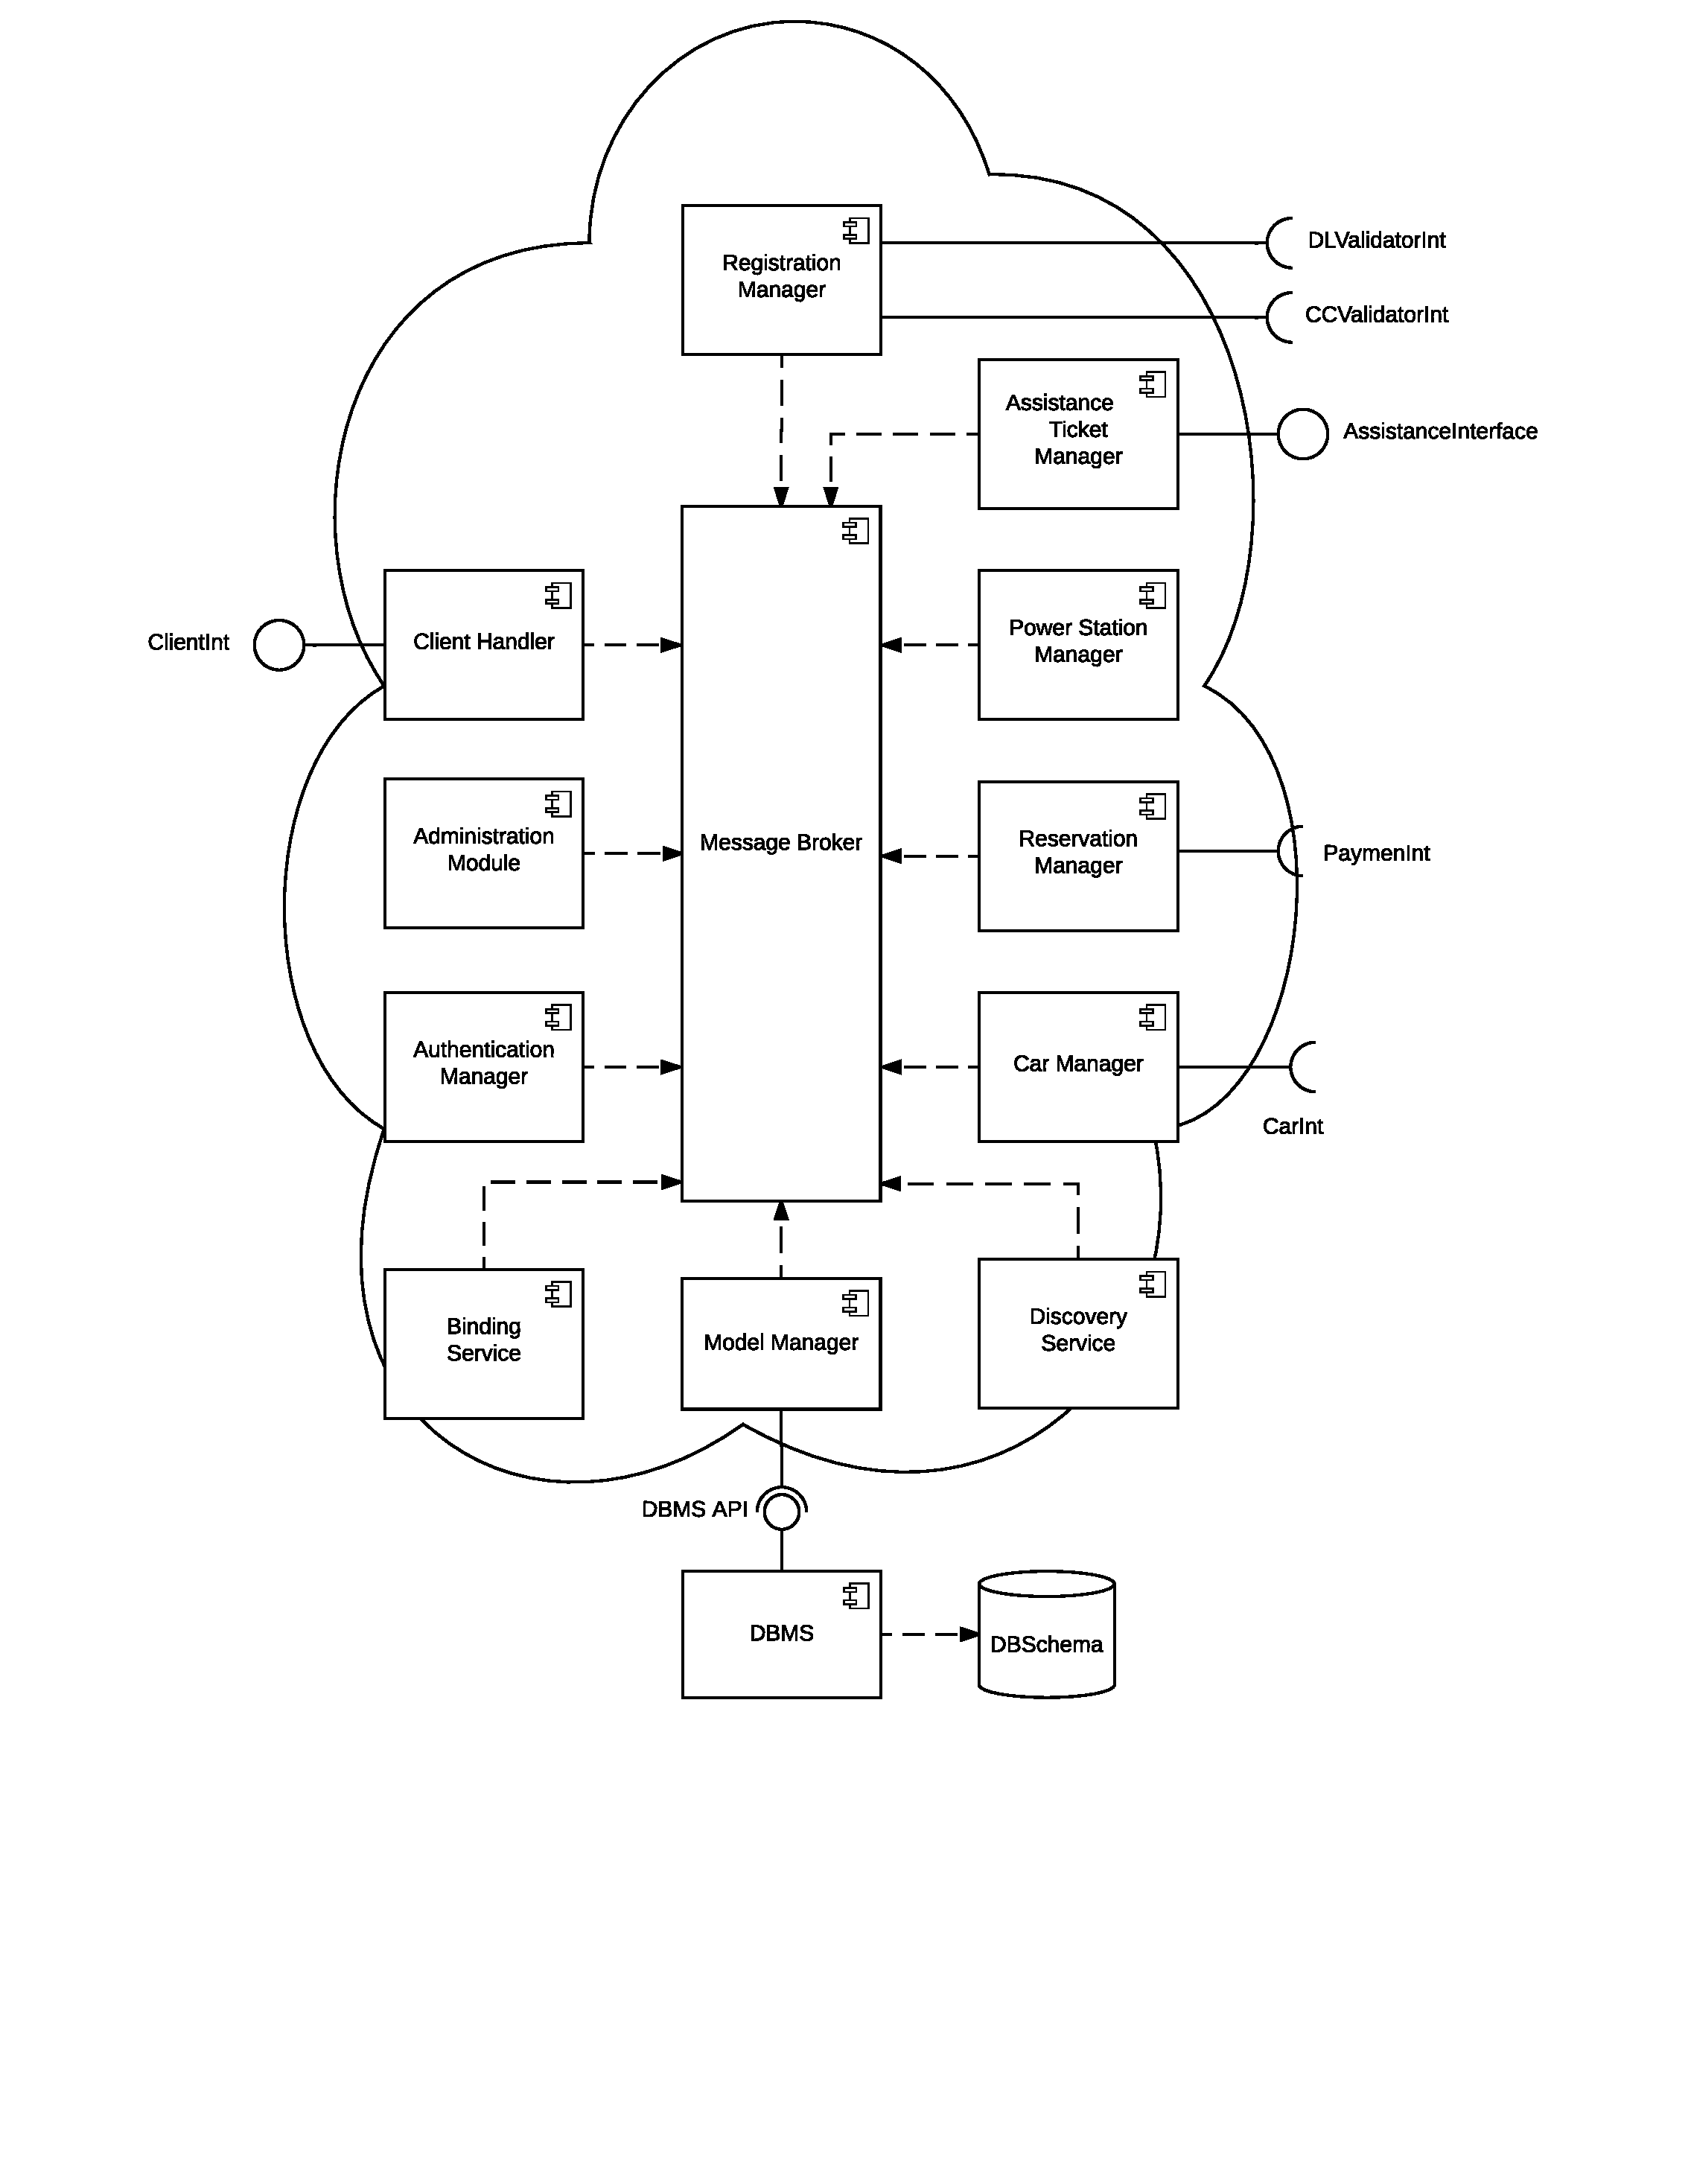
\includegraphics[width=1\textwidth]{ComponentDiagram}

\caption{Component View of the server side single services}
\end{figure}

As previously said the system has been designed in order to respect
the principles of microservice architecture. Therefore every component
will be stateless, independently deployable, able to deal with a specific
aspect of our business domain and to hide to the other services any
kind of implementation detail. 

The communication between these microservices will use AMQP (Advanced
Messaging Queue Protocol) and will be managed by a centralized message
broker (such as RabbitMQ or ActiveMQ). When a new instance of a service
is created the message broker will be automatically connected to the
new service and will publish its existence to the other services through
the ``discovery service'', then the ``binding service'' will take
charge of setting up the correct queue binding rules with the message
broker. That will allow some advanced traffic routing features including
per-version weighting and elastic load balancing on the different
instances of the same service.

The hereunder specified components could be in the future divided
in much more granular services in order to decouple even more their
functionalities:
\begin{itemize}
\item Client Handler: orchestrates the needed services for the clients,
translating REST HTTP requests into AMQP-compliant messages and sending
them to the different microservices as needed.
\item Discovery Service: gives to other services the references that allow
them to communicate with each other.
\item Binding Service: manages the queue binding for the services.
\item Authentication Manager: ensures that only authorised users are able
to perform ``restricted'' actions as well as checking login credentials.
\item Registration Manager: manages the registration of new users and the
update of registered users' data if needed.
\item Administration Module: grants PowerEnJoy's operators access to some
specific features needed to manage the assistance tickets they have
to take care of.
\item Model Manager: grants access to the data to the other components,
abstracting any kind of technology specific detail to the other services.
\item Car Manager: manages the physical cars providing other services with
the needed functionalities and informations.
\item Power Station Manager: manages the physical power stations' data and
functionalities.
\item Assistance Ticket Manager: grants the assistance callcenter, the operators
and the other services the APIs to manage the assistance tickets.
\item Reservation Manager: manages the whole reservation process for an
Active User from the reservation intention to the effective payment,
interacting with the external payment handler through his APIs.
\end{itemize}
All the communications between the different components will be asynchronous
in order to minimise unneeded resource consumption that would result
in an increase of the costs for the commissioner.

Each of these services can be instantiated and deallocated as many
times as needed to handle the momentary load of the system, taking
advantage of the queuing system offered by the message broker. This,
coupled with a dynamic cloud infrastructure that allows quasi-immediate
upscale of computing and networking capability, will allow the system
to handle load spikes along with mitigating the risk of a downtime
due to the excessive load. 

\subsection{Deployment View}

To reach our goals we have depicted 4 main components to be deployed
separately from the numerous services we previously indicated in section
2.2: 
\begin{itemize}
\item Onboard Car Management system: it allows the server and the car to
communicate, and more specifically makes it possible for the server
to retrieve important data from the car and to remotely access car
functions such as locking and unlocking the doors. 
\item PowerStation Data System: it will be deployed in each Power Station
and will manage the communication with the central system ensuring
that every service is able to access relevant data.
\item Mobile App: it will give both operators and Active Users access to
the specific features they have permission to access, only after they
sign in. There are many possible implementations for the app, while
the communication with the Client Handler (on the server) will use
RESTful APIs. Maps will be downloaded from an external probider in
order to have a user-friendly visualization of cars' positions.
\item Web Page: it will allow Visitors to check the map only, while letting
Users reserve cars and change their account's data.
\end{itemize}
\begin{figure}[H]
\includegraphics[width=1\textwidth]{\string"Deployment Diagram\string".pdf}

\caption{Deployment View of the system }
\end{figure}

\pagebreak{}

\subsection{Runtime View}

The following sequence diagrams will only show the way the system
will act while performing certain tasks. They are not meant to be
an exact representation of the software implementation of the procedures.
For sake of simplicity we have preferred to show the intention of
the calls to other services, omitting all the technical details concerning
the mere technological choice of a specific message broker.
\begin{flushleft}
Sign up sequence diagram:
\par\end{flushleft}

\begin{center}
\includegraphics[scale=0.3]{\string"Sequence Diagrams/sequenceSignUp\string".pdf}
\par\end{center}

\begin{flushleft}
Car reservation sequence diagram:
\par\end{flushleft}

\begin{center}
\includegraphics[scale=0.3]{\string"Sequence Diagrams/ReserveCar\string".pdf}
\par\end{center}

\pagebreak{}

End of a car rental:
\begin{center}
\includegraphics[scale=0.3]{\string"Sequence Diagrams/EndRentalInsideSafeZone\string".pdf}
\par\end{center}

\subsection{Component Interfaces}

Seen that we have adopted a message based communication between our
services, the only type of interface with the outside world they need
are the ones defined by the message broker in order to be able to
receive and pull messages from the queues.

The client Handler will offer the necessary REST APIs to the clients.

\subsection{Selected Architectural Styles And Patterns}

As previously stated our system will adopt a 3-tier, cloud-based architecture.
This will allow to decouple the presentation logic from the business
logic as well as to have a shared database management that will be
provided by a PaaS and will be accessed through a single model manager
service, allowing the other services to be stateless.

The overall serverside system will be composed of microservices. The
webserver will take advantage of a fa�ade pattern offered by the ClientHandler
that will work as an API gateway for both the web server and the client
(either a mobile application or a web page). This pattern choice will
allow access to our application without too strict hardware constraints
on user's devices. If needed the system could be made elastic by adding
a service as an ``elastic component'' managing the other services
instantiation. The elastic load balancing will be managed by the API
gateway and the message broker in order to minimize the use of physical
resources and costs.The system will apply a server-side discovery
pattern thanks to the discovery and binding services that will grant
the necessary connection between the various components in a sort
of publish-subscribe pattern where the services are subscribed by
the binding service to the appropriate messaging queue and can publish
to other. The communication between server and client will adopt a
REST architectural style that will allow the decoupling between the
two sides and will give them a common language that allows the developers
to choose the most suitable technology on both sides.

\subsection{Data management}

Although we have used a microservice approach for the business logic
tier, it doesn't make much sense to split data between the different
modules. In fact our data model is very small and interconnected and
we don't need to use different approaches (eg. SQL and noSQL at the
same time). Of course in this way we couple the different modules
but it is inevitable since they run for the same macro-functionality.
A unique database grants us the possibility to ensure in a simple
way ACID properties and to use the standardized SQL language for queries.
We provide an Entity-Relationship model for our application in figure
4.

\begin{figure}
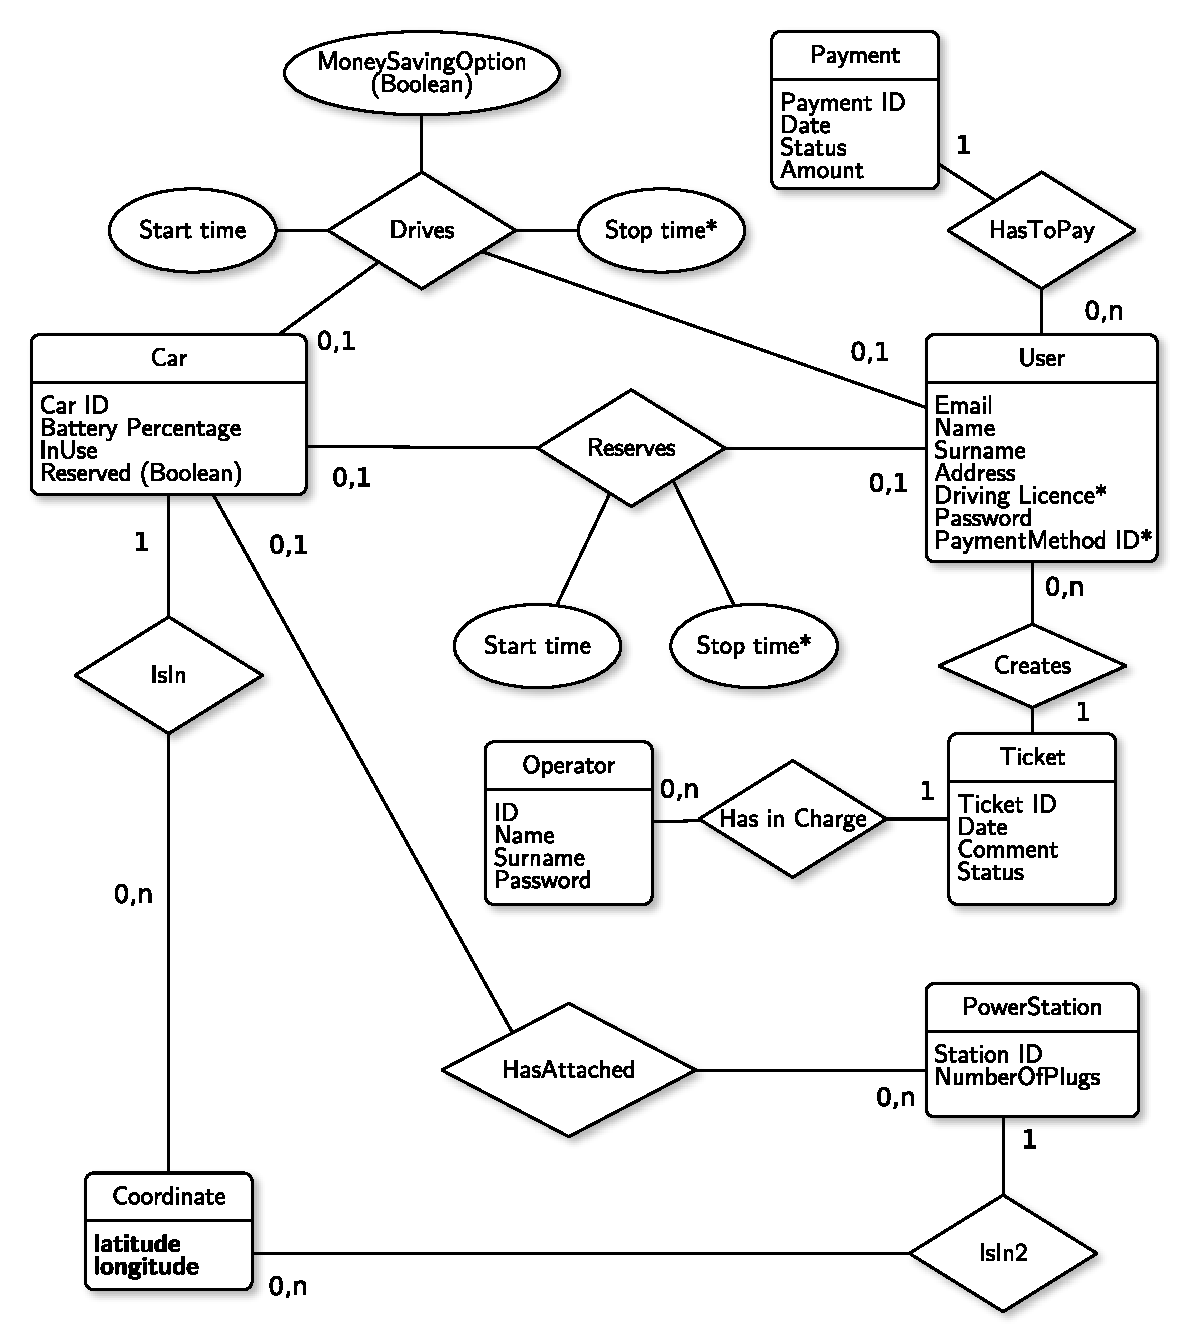
\includegraphics[scale=0.7]{ER}

\caption{ER data model}

\end{figure}


\subsection{Other Design Decisions}

Having taken into account the decisions explained in the previous
sections we decided to implement the overall logic of the system in
Java. We will use Java EE with Frameworks such as Spring Boot as well
as open source services such as RabbitMQ as Message Broker and other
to cover the discovery and binding services, the ClientHandler and
the Authentication Manager. The web server part could be managed by
Nginx in order to reach the needed scalability and reliability and
manage the web interface for the clients.

\pagebreak{}

\section{Algorithm Design}

All algorithms needed in the project are trivial but the one dealing
with uniform repartition of cars in the city.

Cars are picked up by by users in one location dropped off in another
one. Of course the distribution of picking up and dropping off locations
is not uniform. So some operators are needed in order to perform some
relocations, in particular during the night, so that in the morning
cars are located where there is actual necessity. The money saving
option tries to drop the load of relocations, stimulating users to
park where there is a deficiency, with a discount. So the global situation
have to be monitored in real time, taking into account, the static
situation, the reservations and and the current rides.

This problem has been studied a lot and there are in literature various
algorithms that solve it. They are mainly based on mixed integer linear
programming techniques and in particular {[}1{]} presented a complete
model. In {[}2{]} is presented a greedy algorithm that achieves almost
the same result. In {[}3{]} a more sofisticated approach is used taking
into account a three dimensional objective function and exploiting
genetic algorithms and local search methods. {[}4{]} offers a sort
of classification of the strategies proposed in the past years.

For our purpose the approach described in {[}2{]} is the best since
it minimizes the number of the operators needed to relocate cars and
so the costs.

\subsection*{Riferimenti}

{[}1{]} A. G. Kek, R. L. Cheu, Q. Meng, and C. H. Fung, \textquotedblleft A
decision support system for vehicle relocation operations in carsharing
systems'', Transportation Research Part E: Logistics and Transportation
Review, vol. 45, no. 1, pp. 149\textendash 158, 2009.

{[}2{]} R. Zakaria, L. Moalic, A. Caminada, M. Dib, ``A Greedy Algorithm
for relocation problem in one-way carsharing'', 10th International
Conference on Modeling, Optimization and Simulation - MOSIM\textquoteright 14
\textendash{} November 5-7-2014- Nancy \textendash{} France \textquotedblleft Toward
circular Economy\textquotedblright .

{[}3{]} Moalic, L., Lamrous, S., \& Caminada, A. (2013). A Multiobjective
Memetic Algorithm for Solving the Carsharing Problem. Proceedings
Of The 2013 International Conference On Artificial IntelligenceIcai
2013, Vol. 1, pp. 877-883.

{[}4{]} S. Weikl, K. Bogenberger, ``Relocation Strategies and Algorithms
for free-floating Car Sharing Systems'', 15th International IEEE
Conference on Intelligent Transportation Systems Anchorage, Alaska,
USA, September 16-19, 2012.

\pagebreak{}

\section{User Interface Design}

Below are some mockups to show how users will interact with the service.
Since PowerEnJoy can be used both from a computer (except for unlocking
the car), both Mobile and Web mockups are provided. Moreover, since
both Users and Operators have access to the service via browser and
app, interfaces for both types of users have been created. 

\subsection{User Experience Diagram}

This diagram briefly sums up the core interactions that a User can
have with the system, highlighting how each ``Page'' (called Screen)
is accessible in a normal browsing behaviour. A Screen represents
both a Web Page and a Mobile App page since the interactions themselves
do not change. 
\begin{center}
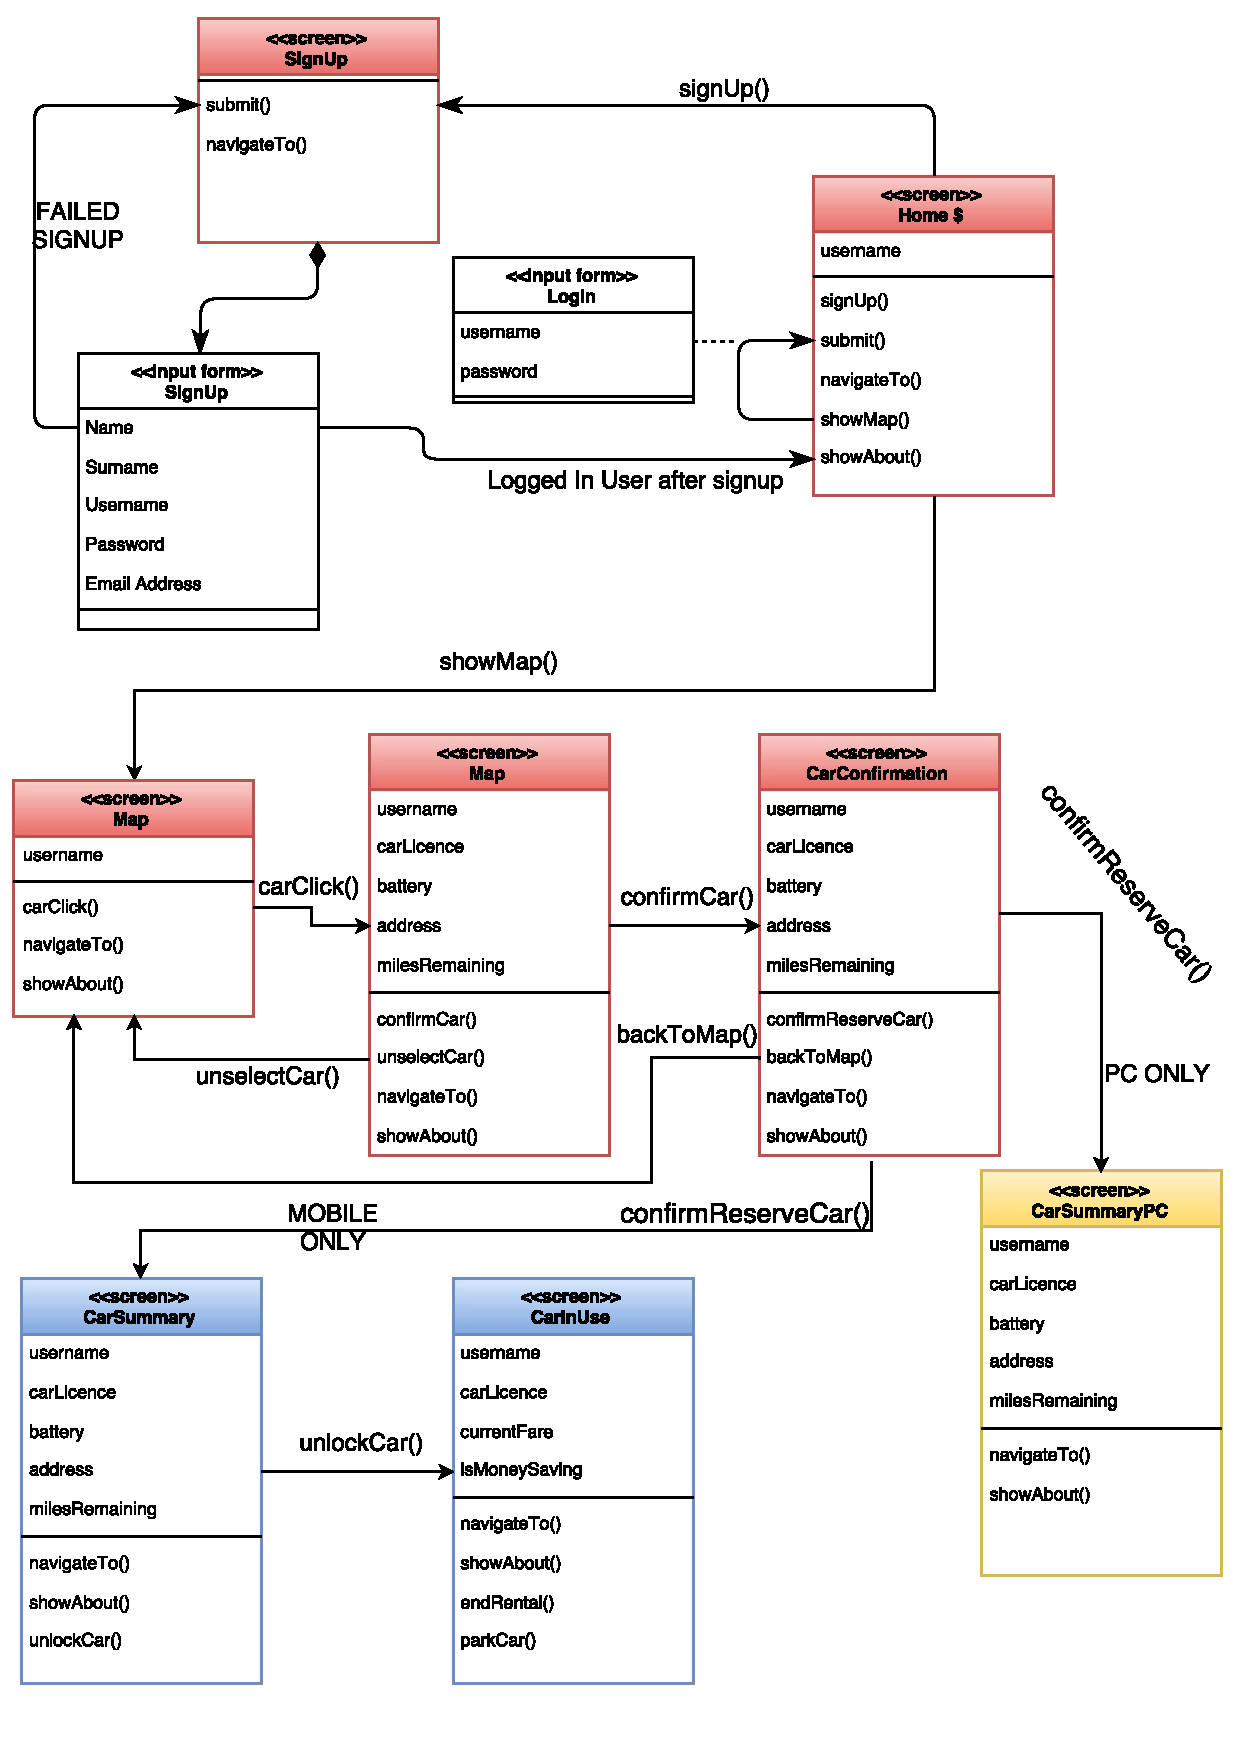
\includegraphics[clip,scale=0.57]{UX}
\par\end{center}

\subsection{User Interfaces}

As anticipated, in this section all User mockups are analyzed. These
mockups show how all actions that can be performed by our users. This
section is further split between Web interfaces, imagined for standard
browsers, and Mobile interfaces, designed having a smartphone App
in mind.

\subsubsection{Web Interfaces}

\paragraph{Home Page (Web)}

From the home page any user can try to login inserting username and
password or they can choose to sign up and go to the registration
page. This page will likely show a description of the service as well
as providing links to other important part of the website (Map, Pricing,
About Us).

\bigskip{}

\begin{center}
\includegraphics[scale=0.6]{\string"Mockup_Exported/PC Home Web\string".png}
\par\end{center}

\pagebreak{}

\paragraph{Registration Page (Web)}

In this page users must input the core informations to register online:
name, surname, email address and username.

\bigskip{}

\begin{center}
\includegraphics[scale=0.6]{\string"Mockup_Exported/PC Sign Up Web\string".png}
\par\end{center}

\paragraph{Further Information (Web)}

After having registered and logged in, users must input their Licence
and Credit Card in order to use the service if they haven't already. 

\bigskip{}

\begin{center}
\includegraphics[scale=0.6]{\string"Mockup_Exported/PC Further Account Info Web\string".png}
\par\end{center}

\pagebreak{}

\paragraph{Map (Web)}

All users can view available cars near their position and choose one
if they want more info (see next mockup).

\bigskip{}

\begin{center}
\includegraphics[scale=0.5]{\string"Mockup_Exported/PC Map Web\string".png}
\par\end{center}

\paragraph{Map - Selected Car (Web)}

Selecting a car provides relevant information about that specific
car, in order to give to the user the chance to pick a car that can
suit his needs. 

\bigskip{}

\begin{center}
\includegraphics[scale=0.5]{\string"Mockup_Exported/PC Map Web - Selected Car\string".png}
\par\end{center}

\pagebreak{}

\paragraph{Selected Car Confirmation (Web)}

After having selected a car and having pressed ``Click to reserve'',
users are asked to confirm their choice one last time, to avoid errors
in case of mistakenly pressed links or misread information.

\bigskip{}

\begin{center}
\includegraphics[scale=0.6]{\string"Mockup_Exported/PC Car confirmation Screen\string".png}
\par\end{center}

\paragraph{Reservation Confirmed (Web)}

Confirming a reservation shows a brief summary containing the address
at which the car is parked. 

\bigskip{}

\begin{center}
\includegraphics[scale=0.6]{\string"Mockup_Exported/PC Car confirmation Screen - Confirmed\string".png}
\par\end{center}

\pagebreak{}

\subsubsection{Mobile Interfaces}

\paragraph{Home (Mobile)}

From the App's home page users can either login or create an account.
Login is handled inside the app, while to create an account the user
is redirected to the website. (On the left)

\paragraph{Map (Mobile)}

The user is shown a map displaying all cars that are nearby. His position
can be calculated using the built in GPS receiver or can be manually
input. (On the right)

\bigskip{}

\includegraphics[scale=0.55]{\string"Mockup_Exported/Home Mobile\string".png}\includegraphics[scale=0.55]{\string"Mockup_Exported/Map Mobile\string".png}

\pagebreak{}

\paragraph{Selected Car (Mobile)}

Selecting a car on the map shows relevant information, like it happens
on the website. (On the left)

\paragraph{Car Confirmation (Mobile)}

A user can confirm a reservation or go back if he chose that car by
mistake. (On the right)

\bigskip{}

\includegraphics[scale=0.55]{\string"Mockup_Exported/Selected Car mobile\string".png}\includegraphics[scale=0.55]{\string"Mockup_Exported/Car Confirmation Mobile\string".png}

\pagebreak{}

\paragraph{Reservation Confirmed (Mobile)}

When the reservation is confirmed, the smartphone shows a countdown
as well as the car's address. (On the left)

\paragraph{Car In Use (Mobile)}

While using the car, Users can decide to park it \textemdash{} which
signals the system that the car will be picked up by the same user
and that the rental is not to be terminated \textemdash{} or to end
the rental. (On the right)

\bigskip{}

\includegraphics[scale=0.55]{\string"Mockup_Exported/Car Confirmed Mobile\string".png}\includegraphics[scale=0.55]{\string"Mockup_Exported/Car Park or End Mobile\string".png}

\pagebreak{}

\paragraph{Car Parked (Mobile)}

If the car is already parked users can decide to end the rental using
the app. In case they want to continue their journey, they only have
to jump back on the car. (On the left)

\paragraph{Rental Ended (Mobile)}

Ending a rental shows the total as well as whether the Money Saving
Option was active for the trip. (On the right)

\bigskip{}

\includegraphics[scale=0.55]{\string"Mockup_Exported/Car Parked\string".png}\includegraphics[scale=0.55]{\string"Mockup_Exported/Rental Ended\string".png}

\pagebreak{}

\subsection{Operator Interfaces}

\subsubsection{Web Interfaces}

\paragraph{Operator Main Page (Web)}

Operators can choose between performing a pending task (a ``Todo'')
or managing a specific car.

\bigskip{}

\begin{center}
\includegraphics[scale=0.55]{\string"Mockup_Exported/PC Operator Main\string".png}
\par\end{center}

\paragraph{Operator chose TODO (Web)}

Choosing a pending operation brings up relevant information about
it: its type, the position (if relevant), a short summary and a map.
The operator can confirm the task if he will take care of it or go
back to the home page(the logo links to the home page).

\bigskip{}

\begin{center}
\includegraphics[scale=0.55]{\string"Mockup_Exported/PC Operator chosen TODO\string".png}
\par\end{center}

\pagebreak{}

\paragraph{Operator Searched Car (Web)}

Choosing to manage a specific car allows the operator to search among
all cars, by car Licence Plate or by Current Driver (User) if in use.

\bigskip{}

\begin{center}
\includegraphics[scale=0.6]{\string"Mockup_Exported/PC Operator Choose Car\string".png}
\par\end{center}

\paragraph{Car Details (Web)}

The Car Details page shows all informations available for the chosen
car as well as providing buttons to change all editable parameters
(for instance the car's status).

\bigskip{}

\begin{center}
\includegraphics[scale=0.6]{\string"Mockup_Exported/PC Operator Manage Car\string".png}
\par\end{center}

\pagebreak{}

\paragraph{Changing a Car parameter - Sample (Web)}

Choosing to edit a parameter brings up a ``pop-up'' providing the
needed options to edit.

\bigskip{}

\begin{center}
\includegraphics[scale=0.6]{\string"Mockup_Exported/PC Operator Car Specific Operation (Sample)\string".png}
\par\end{center}

\pagebreak{}

\subsubsection{Mobile Interfaces}

\paragraph{Main Page (Mobile)}

The mobile Main page for operators offers the same options of the
web one: they caan either choose a pensing task or opt to manage a
car. (On the left)

\paragraph{Operator chose TODO (Mobile)}

(On the right)

\bigskip{}

\includegraphics[scale=0.55]{\string"Mockup_Exported/Operator Main Mobile\string".png}\includegraphics[scale=0.55]{\string"Mockup_Exported/Operator Chosen TODO Mobile\string".png}

\pagebreak{}

\paragraph{Operator Searched Car (Mobile)}

(On the left)

\paragraph{Operator Car Details (Mobile)}

(On the right)

\bigskip{}

\includegraphics[scale=0.55]{\string"Mockup_Exported/Operator Choose Car Mobile\string".png}\includegraphics[scale=0.55]{\string"Mockup_Exported/Operator Manage Car Mobile\string".png}

\pagebreak{}

\paragraph{Changing a Car parameter - Sample (Mobile)}

\bigskip{}

\begin{center}
\includegraphics[scale=0.6]{\string"Mockup_Exported/Operator Manage Car Specific Mobile\string".png}
\par\end{center}

\pagebreak{}

\subsection{Car Interface}

\subsubsection{Car Screen}

The car has a screen that shows the fare in real time as well as showing
whether the Money Saving Option is active or not.

\bigskip{}

\begin{center}
\includegraphics[scale=0.8]{\string"Mockup_Exported/On-board screen\string".png}
\par\end{center}

\pagebreak{}

\section{Requirements traceability}

Below are listed all requirements defined in our RASD and their mapping
on the architecture. The map is neither injective nor surjective.
In fact some requirements need more than one module to be satisfied
and modules achieve the satisfiability of many requirements.

\begin{longtable}{|>{\raggedright}p{0.5cm}|>{\raggedright}p{6.5cm}|>{\raggedright}p{6cm}|}
\hline 
\# & \textbf{Requirement} & \textbf{Mapping on the architecture}\tabularnewline
\endhead
\hline 
\multicolumn{3}{|c|}{\textbf{G1: Allow visitors to sign up}}\tabularnewline
\hline 
1 & A valid email is required during the registration. & Registration manager\tabularnewline
\hline 
2 & A valid DL is required. & Registration manager + DL validator\tabularnewline
\hline 
3 & Invalid emails are all addresses that are either already in use or
not well formed. & Registration manager\tabularnewline
\hline 
4 & Email Address must be verified. & Registration manager\tabularnewline
\hline 
5 & The DL is valid if all the fields match the user\textquoteright s
information and the Licence Office confirms that the Licence Number,
the Name and the Surname are correct. & Registration manager + DL validator\tabularnewline
\hline 
6 & Foreign DL must be verified by an Operator. & DL validator + Assistance ticket manager + Administration module\tabularnewline
\hline 
7 & If some of the provided information is incorrect, the registration
is rejected and the user is prompted to fix the issue(s). & Registration manager\tabularnewline
\hline 
\multicolumn{3}{|c|}{\textbf{G2: Allow visitors to log in}}\tabularnewline
\hline 
8 & A previously registered email is required. & Autentication manager\tabularnewline
\hline 
9 & The password chosen during the registration of the submitted email
has to be inserted in order to log in. & Autentication manager\tabularnewline
\hline 
10 & Visitors submitting incorrect email and/or password shall not be allowed
to log in. & Autentication manager\tabularnewline
\hline 
\multicolumn{3}{|c|}{\textbf{G3: Allow Users to update or modify their profile's information}}\tabularnewline
\hline 
11 & Every registered User can modify his information. & Autentication manager + Registration manager\tabularnewline
\hline 
12 & Changing email address is allowed but the new email must be confirmed
for the account to be valid. & Autentication manager + Registration manager\tabularnewline
\hline 
13 & Changing the CC information is allowed as long as the new CC is valid. & Registration manager + CC validator\tabularnewline
\hline 
14 & Changing the DL is allowed but the Licence has to be verified. & Registration manager + DL validator\tabularnewline
\hline 
15 & Changing name and/or surname is not allowed. & Registration manager\tabularnewline
\hline 
\newpage
\hline 
\multicolumn{3}{|c|}{\textbf{G4: Show updated information on available cars}}\tabularnewline
\hline 
16 & The list of available cars always includes only cars that are parked
and not reserved and is shown on a map in the location where it is
actually parked. & Car manager + Reservation manager\tabularnewline
\hline 
17 & If a car is reserved is tagged on the map as reserved. & Car manager + Reservation manager\tabularnewline
\hline 
18 & For every car is displayed the remaining percentage of the battery. & Car manager\tabularnewline
\hline 
19 & Users should be able to apply filters to show only cars within a certain
distance from a specified location or with a minimum percentage of
battery left. & Car manager + Model manager\tabularnewline
\hline 
\multicolumn{3}{|c|}{\textbf{G5: Allow Active Users to reserve a car}}\tabularnewline
\hline 
20 & Only Active Users can reserve cars. & Autentication manager + Reservation manager\tabularnewline
\hline 
21 & Cars can be reserved by a specific user for up to one hour before
being unlocked. & Car manager + Reservation manager\tabularnewline
\hline 
22 & If a reserved car is not unlocked in one hour the reservation expires
and the user pays a fine of 1�. & Reservation manager\tabularnewline
\hline 
23 & Only available cars can be reserved. & Reservation manager\tabularnewline
\hline 
24 & If an active user is already using a car he cannot reserve another
one. & Reservation manager\tabularnewline
\hline 
25 & The system shall provide the user the possibility to delete his pending
reservation. & Reservation manager\tabularnewline
\hline 
26 & The deletion of a reservation shall be allowed only before the reserved
car has been unlocked. & Reservation manager + Car manager\tabularnewline
\hline 
\multicolumn{3}{|c|}{\textbf{G6: Allow Active Users to unlock the car they reserved}}\tabularnewline
\hline 
27 & A car can be unlocked only by the user who has reserved it. & Reservation manager + Car manager\tabularnewline
\hline 
28 & There exists a mechanism of acknowledgment between the car and the
user. & Car management system + Car manager + Reservation manager\tabularnewline
\hline 
29 & The car is unlocked only after the user is acknowledged. & Car management system + Car manager\tabularnewline
\hline 
30 & If a user unlocks the car without igniting the engine, the systems
starts charging the regular price after the pick up time (one hour
from the reservation) expires. & Car management system + Car manager + Reservation manager\tabularnewline
\hline 
31 & If a user does not ignite the car within 15 minutes from the moment
he unlocks it, the systems prompts the user to confirm he is fine.
If no answer is received, an operator checks the car. & Car management system + Car manager + Reservation manager + Administration
module\tabularnewline
\hline 
\multicolumn{3}{|c|}{\textbf{G7: Compute the fare}}\tabularnewline
\hline 
32 & The fare takes into account all price modifiers (discounts or extra
fees). & Reservation manager\tabularnewline
\hline 
33 & The computed fare is based on how many minutes have passed since the
engine was ignited. & Reservation manager + Car management system\tabularnewline
\hline 
34 & If the engine was never ignited the fare is calculated as explained
in R30. & Car management system + Car manager + Reservation manager\tabularnewline
\hline 
35 & The computed fare is shown real-time on the car\textquoteright s screen. & Car management system + Car manager + Reservation manager\tabularnewline
\hline 
36 & The system shall be able to apply predetermined discounts to users
following some predetermined behavior. & Reservation manager\tabularnewline
\hline 
37 & The system shall be able to know the number of passengers into a specific
rented car. & Car management system + Car manager\tabularnewline
\hline 
38 & The system shall be able to know the battery percentage of a specific
car in any moment. & Car management system + Car manager\tabularnewline
\hline 
39 & The system shall be able to locate a car and know whether or not it
is plugged at one of the predetermined parking areas in any moment. & Car management system + Car manager + Power station manager\tabularnewline
\hline 
40 & The system shall be able to measure the distance of a specific car
from the nearest power grid station. & Car management system + Car manager + Power station manager\tabularnewline
\hline 
41 & The system shall be able to make an Operator charge a specific car. & Car management system + Car manager + Power station manager + Administration
module\tabularnewline
\hline 
42 & The system shall know if a user selected the money saving option. & Reservation maanager\tabularnewline
\hline 
\multicolumn{3}{|c|}{\textbf{G8: Allow System Administrator(s) to update information}}\tabularnewline
\hline 
43 & The System Administrator is granted the necessary permissions allowing
him to access each cars\textquoteright{} data, status and position. & Autentication manager\tabularnewline
\hline 
44 & The system shall present an Interface for the System Administrator
in order to access with the necessary permissions. & Autentication manager\tabularnewline
\hline 
45 & Only those accessing the systems with these permissions shall be able
to access sensible data regarding the cars. & Autentication manager\tabularnewline
\hline 
46 & The system shall be able to check the consistency of the information
modified given a set of rules. & Model manager\tabularnewline
\hline 
\multicolumn{3}{|c|}{\textbf{G9: Ensure that the fare is paid}}\tabularnewline
\hline 
47 & As soon as the rental is ended, use the payment method provided by
the AU to pay the fare. & Reservation manager + Payment Handler\tabularnewline
\hline 
48 & If the provided method is invalid (e.g. expired or empty CC), notify
the user. & Reservation manager + Payment Handler\tabularnewline
\hline 
49 & Users with unsuccessful pending fare shall not be allowed to book
cars. & Reservation manager\tabularnewline
\hline 
50 & Allow users to specify the main payment method. & Registration manager\tabularnewline
\hline 
51 & Periodically try to charge pending fare through the specified main
payment method. & Reservation manager + Payment Handler\tabularnewline
\hline 
\multicolumn{3}{|c|}{\textbf{G10: Allow the driver to choose the money saving option}}\tabularnewline
\hline 
52 & The systems suggests a charging station near the user\textquoteright s
destination if present (within a user-selectable radius). & Reservation manager\tabularnewline
\hline 
53 & The suggested station must have at least a free plug to be suggested. & Reservation manager\tabularnewline
\hline 
54 & The suggested station shall be determined to ensure a uniform distribution
of cars. & Car manager\tabularnewline
\hline 
55 & If the AU doesn\textquoteright t park in the suggested station the
money saving option shall not be taken into account for future decisions. & Reservation manager\tabularnewline
\hline 
56 & If the AU chooses this option, the system gives him the address and
shows directions on the smartphone. & Reservation manager\tabularnewline
\hline 
\multicolumn{3}{|c|}{\textbf{G11: Allow the user to park the rented car in safe zone}}\tabularnewline
\hline 
57 & Parking shall be allowed only in safe zones. & Reservation manager\tabularnewline
\hline 
58 & The system shall not charge the user after the car has been parked
and he has exited the car. & Reservation manager + Car manager + Car management system\tabularnewline
\hline 
59 & The system shall lock the car, if parked in a safe area and the user
has exited the car. & Reservation manager + Car manager + Car management system\tabularnewline
\hline 
60 & The system shall be able to recognize whether or not there is a user
inside the car. & Car manager + Car management system\tabularnewline
\hline 
\end{longtable}

The corrispondence is summarized in the following figure.
\begin{center}
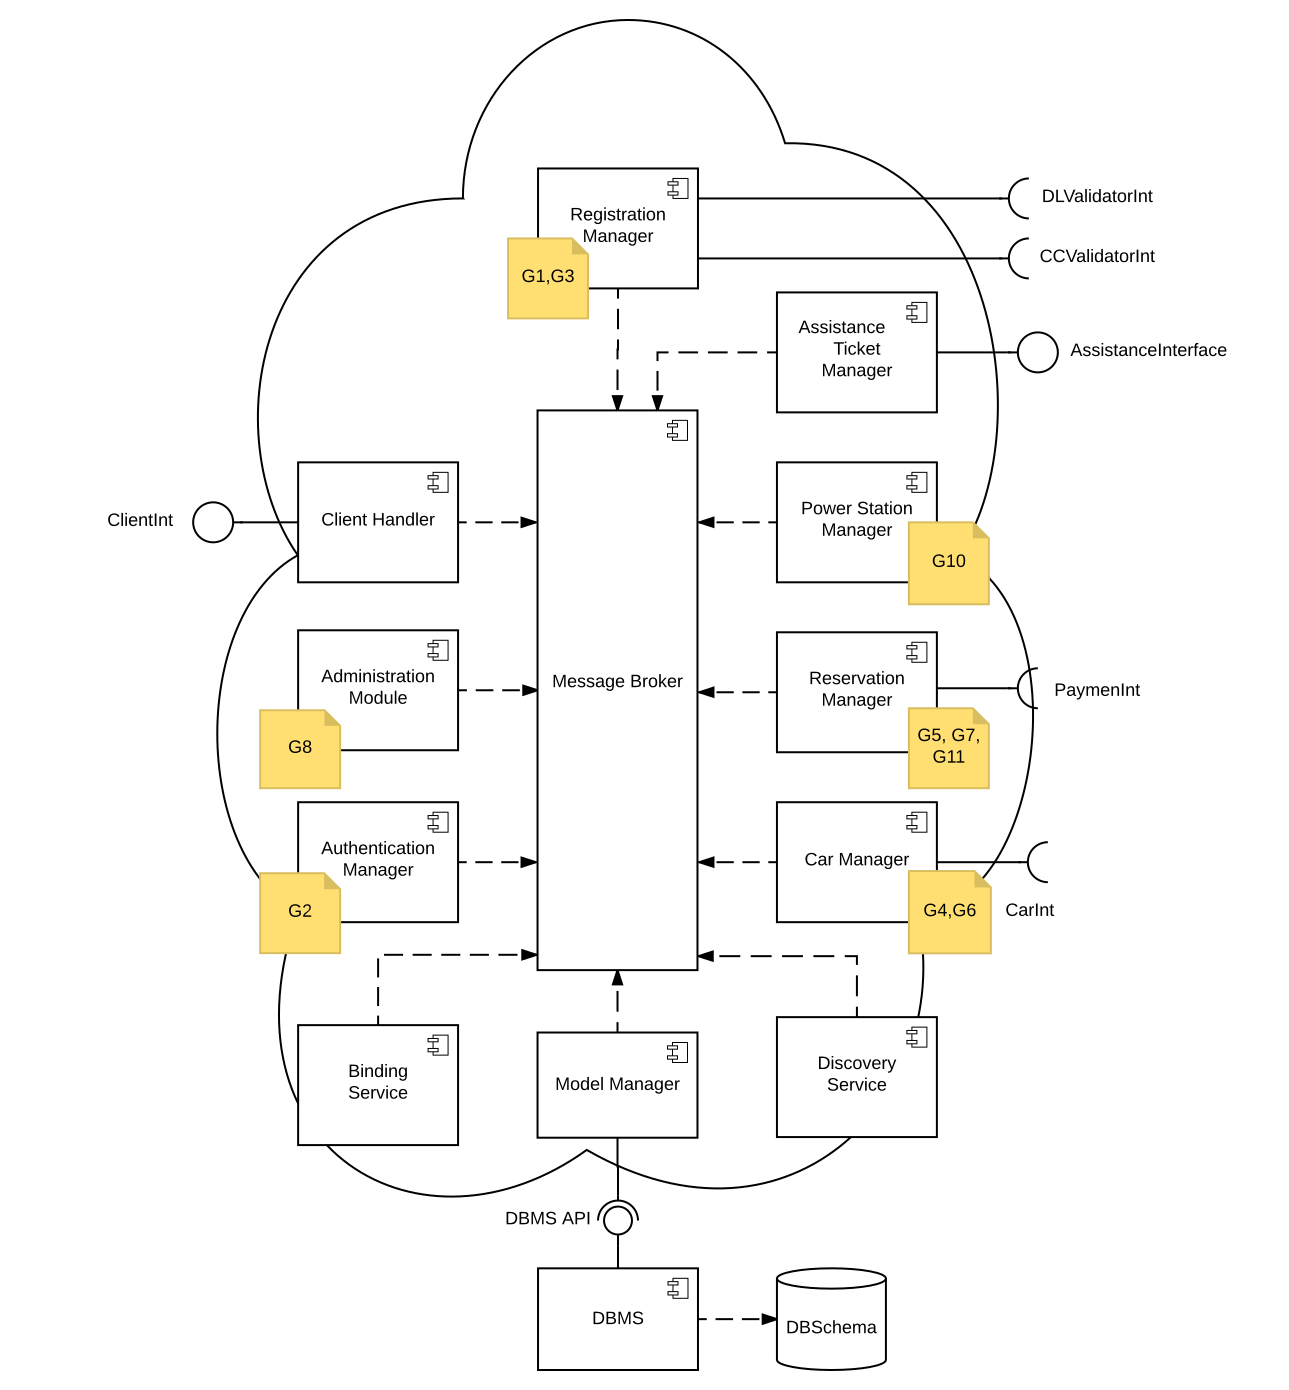
\includegraphics[scale=0.4]{ComponentDiagramGoals}
\par\end{center}

\section{Effort spent}

\begin{tabular}{|c|c|}
\hline 
\textbf{Component} & \textbf{Time spent (in hour)}\tabularnewline
\hline 
\hline 
Philippe Scorsolini & 35\tabularnewline
\hline 
Lorenzo Semeria & 22\tabularnewline
\hline 
Gabriele Vanoni & 22\tabularnewline
\hline 
\end{tabular}

\section{References}
\begin{itemize}
\item https://www.rabbitmq.com/documentation.html
\item http://microservices.io/patterns/apigateway.html
\item http://microservices.io/patterns/microservices.html
\item http://microservices.io/patterns/data/shared-database.html
\item http://microservices.io/patterns/microservice-chassis.html
\item http://projects.spring.io/spring-boot/
\item https://www.adayinthelifeof.nl/2011/06/02/asynchronous-operations-in-rest/
\item https://spring.io/blog/2015/07/14/microservices-with-spring
\item https://sudo.hailoapp.com/services/2015/03/09/journey-into-a-microservice-world-part-2/
\item https://www.nginx.com/blog/introduction-to-microservices/?utm\_source=deploying-microservices\&utm\_medium=blog\&utm\_campaign=Microservices
\item http://www.cloudcomputingpatterns.org/
\item https://www.amqp.org/
\item http://mqtt.org/
\item http://brunorocha.org/python/microservices-with-python-rabbitmq-and-nameko.html
\item http://www.slideshare.net/chris.e.richardson/developing-apps-with-a-microservice-architecture-svforum-microservices-meetup
\item https://docs.microsoft.com/en-us/azure/service-bus-messaging/service-bus-amqp-overview
\item http://projects.spring.io/spring-cloud/
\item http://nordicapis.com/api-gateways-direct-microservices-architecture/
\item https://www.nginx.com/blog/introducing-the-nginx-microservices-reference-architecture/
\item https://www.nginx.com/blog/adopting-microservices-at-netflix-lessons-for-team-and-process-design/
\item https://msdn.microsoft.com/en-us/library/dn568099.aspx
\item https://sudo.hailoapp.com/web/2014/12/08/webapps-as-microservices/
\item https://github.com/mfornos/awesome-microservices
\end{itemize}

\section{Changelog}
\begin{itemize}
\item 28/12/2016 added section 1: design process explanation
\end{itemize}

\end{document}
